\documentclass[a4paper,11pt]{article}
\usepackage{amsmath,amsthm,amsfonts,amssymb,amscd,amstext,vmargin,graphics,graphicx,tabularx,multicol} 
\usepackage[francais]{babel}
\usepackage[utf8]{inputenc}  
\usepackage[T1]{fontenc} 
\usepackage{pstricks-add,tikz,tkz-tab,variations}
\usepackage[autolanguage,np]{numprint} 
\usepackage{calc}
\usepackage{mathrsfs}

\usepackage{cancel}

\setmarginsrb{1.5cm}{0.5cm}{1cm}{0.5cm}{0cm}{0cm}{0cm}{0cm} %Gauche, haut, droite, haut
\newcounter{numexo}
\newcommand{\exo}[1]{\stepcounter{numexo}\noindent{\bf Exercice~\thenumexo} : }
\reversemarginpar

\newcommand{\bmul}[1]{\begin{multicols}{#1}}
\newcommand{\emul}{\end{multicols}}

\newcounter{enumtabi}
\newcounter{enumtaba}
\newcommand{\q}{\stepcounter{enumtabi} \theenumtabi.  }
\newcommand{\qa}{\stepcounter{enumtaba} (\alph{enumtaba}) }
\newcommand{\initq}{\setcounter{enumtabi}{0}}
\newcommand{\initqa}{\setcounter{enumtaba}{0}}

\newcommand{\be}{\begin{enumerate}}
\newcommand{\ee}{\end{enumerate}}
\newcommand{\bi}{\begin{itemize}}
\newcommand{\ei}{\end{itemize}}
\newcommand{\bp}{\begin{pspicture*}}
\newcommand{\ep}{\end{pspicture*}}
\newcommand{\bt}{\begin{tabular}}
\newcommand{\et}{\end{tabular}}
\renewcommand{\tabularxcolumn}[1]{>{\centering}m{#1}} %(colonne m{} centrée, au lieu de p par défault) 
\newcommand{\tnl}{\tabularnewline}

\newcommand{\trait}{\noindent \rule{\linewidth}{0.2mm}}
\newcommand{\hs}[1]{\hspace{#1}}
\newcommand{\vs}[1]{\vspace{#1}}

\newcommand{\N}{\mathbb{N}}
\newcommand{\Z}{\mathbb{Z}}
\newcommand{\R}{\mathbb{R}}
\newcommand{\C}{\mathbb{C}}
\newcommand{\Dcal}{\mathcal{D}}
\newcommand{\Ccal}{\mathcal{C}}
\newcommand{\mc}{\mathcal}

\newcommand{\vect}[1]{\overrightarrow{#1}}
\newcommand{\ds}{\displaystyle}
\newcommand{\eq}{\quad \Leftrightarrow \quad}
\newcommand{\vecti}{\vec{\imath}}
\newcommand{\vectj}{\vec{\jmath}}
\newcommand{\Oij}{(O;\vec{\imath}, \vec{\jmath})}
\newcommand{\OIJ}{(O;I,J)}


\newcommand{\reponse}[1][1]{%
\multido{}{#1}{\makebox[\linewidth]{\rule[0pt]{0pt}{20pt}\dotfill}
}}

\newcommand{\titre}[5] 
% #1: titre #2: haut gauche #3: bas gauche #4: haut droite #5: bas droite
{
\noindent #2 \hfill #4 \\
#3 \hfill #5

\vspace{-1.6cm}

\begin{center}\rule{6cm}{0.5mm}\end{center}
\vspace{0.2cm}
\begin{center}{\large{\textbf{#1}}}\end{center}
\begin{center}\rule{6cm}{0.5mm}\end{center}
}



\begin{document}
\pagestyle{empty}
\titre{Séance d'exercices: Résolution d'équation du premier degré}{}{}{3ème}{}

\vspace*{0.2cm}



 
 
 

\textbf{EXERCICE 5}\\

Noah veut acheter des livres qui coûtent le même prix.\\
S'il en achète 7, il lui manque 1,20 euros. S'il en achète 6, il lui reste 3,50 euros.\\

Quel est le prix d'un livre ?\\


\color{red}
On appelle $x$ le prix d'un livre.\\

L'équation est la suivante : \hspace*{1cm} $7x-1,20= 6x+3,50$ 


$$7x-1,20-6x= 6x+3,50-6x$$

$$x-1,20= 3,50$$

$$x-1,20+1,20=3,50+1,20$$

$$x=4,70$$

Un livre coûte 4,70 euros.\\

 \color{black}
\vspace*{0.5cm}


 
 \textbf{EXERCICE 7}\\

Thomas a obtenu 11 et 16 aux deux premiers contrôles de Maths.\\
Quelle note doit-il avoir au troisième contrôle pour obtenir 15 de moyenne ?\\

\color{red}
On appelle $x$ la troisième note.\\

$$\dfrac{11 + 16 + x}{3}=15$$

$$\dfrac{27 + x}{3}=15$$

$$\dfrac{(27+ x)\times \cancel{3}}{\cancel{3}}=15 \times 3$$


$$27+ x=15 \times 3$$

$$27+ x=45$$

$$27+ x-27=45-27$$

$$ \fbox{ x=18}$$

La troisième note de Thomas doit être un 18 pour obtenir 15 de moyenne.\\

\color{black}

 
\textbf{EXERCICE 8}\\
 \textbf{Trouver la valeur de x pour que l'aire de AMNP soit égale au tiers de l'aire du carré ABCD.}\\
 Justifier votre réponse à l'aide d'une équation.\\


\begin{center}
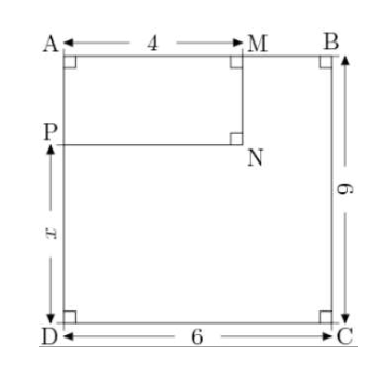
\includegraphics[scale=0.9]{carre.eps} 

\end{center}

\textit{\underline{Indication : } Exprimer l'aire du rectangle AMNP en fonction de x et l'aire du carré ABCD.}\\ 

\color{red}
On appelle $x$ la longueur DP.\\


Dans l'énoncé, il est question de l'aire du rectangle AMNP et de l'aire du carré ABCD.\\
On va donc essayer de les exprimer  :\\

- $A_{ABCD} = 6 \times 6$ \hspace*{1cm} $A_{ABCD} = 6 \times 6 = \underline{36} $ \\

- $A_{AMNP} = L \times l = \underline{4 \times (6-x)}$\\

On trouve donc l'équation suivante : \hspace*{1cm} $A_{AMNP} = \dfrac{A_{ABCD}}{3}$\\

$$4(6-x)=\dfrac{36}{3} $$

$$24-4x=12 $$

$$24-4x -24=12-24 $$

$$-4x = -12 $$

$$\dfrac{-4x}{-4}= \dfrac{-12}{-4} $$

$$ \fbox{x = 3} $$


On trouve donc que pour x = 3, l'aire de AMNP soit égale au tiers de l'aire du carré ABCD.\\


\textbf{Vérification :} \\
- $A_{ABCD} = 6 \times 6 = 36$ \\

- $A_{AMNP} = L \times l = 4 \times 3 = 12$\\

et $36 \div 3 = 12$\\

\color{black}
\vspace*{0.5cm}




\end{document}
